%% abtex2-modelo-artigo.tex, v-1.9.6 laurocesar
%% Copyright 2012-2016 by abnTeX2 group at http://www.abntex.net.br/ 
%%
%% This work may be distributed and/or modified under the
%% conditions of the LaTeX Project Public License, either version 1.3
%% of this license or (at your option) any later version.
%% The latest version of this license is in
%%   http://www.latex-project.org/lppl.txt
%% and version 1.3 or later is part of all distributions of LaTeX
%% version 2005/12/01 or later.
%%
%% This work has the LPPL maintenance status `maintained'.
%% 
%% The Current Maintainer of this work is the abnTeX2 team, led
%% by Lauro César Araujo. Further information are available on 
%% http://www.abntex.net.br/
%%
%% This work consists of the files abntex2-modelo-artigo.tex and
%% abntex2-modelo-references.bib
%%

% ------------------------------------------------------------------------
% ------------------------------------------------------------------------
% abnTeX2: Modelo de Artigo Acadêmico em conformidade com
% ABNT NBR 6022:2003: Informação e documentação - Artigo em publicação 
% periódica científica impressa - Apresentação
% ------------------------------------------------------------------------
% ------------------------------------------------------------------------

\documentclass[
	% -- opções da classe memoir --
	article,			% indica que é um artigo acadêmico
	12pt,				% tamanho da fonte
	oneside,			% para impressão apenas no recto. Oposto a twoside
	a4paper,			% tamanho do papel. 
	% -- opções da classe abntex2 --
	%chapter=TITLE,		% títulos de capítulos convertidos em letras maiúsculas
	section=TITLE,		% títulos de seções convertidos em letras maiúsculas
	subsection=TITLE,	% títulos de subseções convertidos em letras maiúsculas
	%subsubsection=TITLE % títulos de subsubseções convertidos em letras maiúsculas
	% -- opções do pacote babel --
	english,			% idioma adicional para hifenização
	brazil,				% o último idioma é o principal do documento
	sumario=tradicional
	]{abntex2}


% ---
% PACOTES
% ---

% ---
% Pacotes fundamentais 
% ---
% \usepackage{lmodern}			% Usa a fonte Latin Modern
\usepackage{newtxtext, newtxmath} % Usa a fonte Times New Roman

\usepackage[T1]{fontenc}		% Selecao de codigos de fonte.
\usepackage[utf8]{inputenc}		% Codificacao do documento (conversão automática dos acentos)
\usepackage{indentfirst}		% Indenta o primeiro parágrafo de cada seção.
\usepackage{nomencl} 			% Lista de simbolos
\usepackage{color}				% Controle das cores
\usepackage{graphicx}			% Inclusão de gráficos
\usepackage{microtype} 			% para melhorias de justificação
% ---
		
% ---
% Pacotes adicionais, usados apenas no âmbito do Modelo Canônico do abnteX2
% ---
\usepackage{lipsum}				% para geração de dummy text
% ---
		
% ---
% Pacotes de citações
% ---
\usepackage[brazilian,hyperpageref]{backref}	 % Paginas com as citações na bibl
% \usepackage[alf]{abntex2cite}	% Citações padrão ABNT
\usepackage[abnt-emphasize=bf,alf]{abntex2cite}	% Título da citação em negrito
% ---

% ---
% Chiquitto
\usepackage[table,xcdraw]{xcolor}

\newcommand{\autorI}{Alisson G. Chiquitto}
\newcommand{\autorIEmail}{alisson.chiquitto@ifms.edu.br}
\newcommand{\autorII}{André Baida}
\newcommand{\autorIIEmail}{andre.baida@ifms.edu.br}

% https://github.com/eekBR/ufpr-abntex
% \usepackage[style=abnt,backref=true,backend=biber,citecounter=true,backrefstyle=three]{biblatex}

% https://github.com/abntex/abntex2/issues/194
%\usepackage[style=abnt-numeric, comp]{biblatex}
%\usepackage[style=abnt]{biblatex}
%\addbibresource{references.bib}

\graphicspath{{img/}}

% http://benalexkeen.com/correlation-in-python/
% http://www.diaadiaeducacao.pr.gov.br/portals/pde/arquivos/1443-8.pdf

% https://texblog.org/2012/03/21/cross-referencing-list-items/
\makeatletter
\def\namedlabel#1#2{\begingroup
	#2%
	\def\@currentlabel{#2}%
	\phantomsection\label{#1}\endgroup
}
\makeatother

\usepackage{subcaption}

\newcounter{counterResultados}
%\setcounter{counterResultados}{1}
\newcommand{\rtask}[1]{
	\refstepcounter{counterResultados}\label{#1}%
	\arabic{counterResultados} %\stepcounter{counterResultados}
}

% https://github.com/abntex/abntex2/issues/218
\ifthenelse{\equal{\ABNTEXisarticle}{true}}{%
	\renewcommand{\maketitlehookb}{}
}{}

% http://tex.my/customising-running-headers-and-footers/
\makeevenhead{plain}{}{
\includegraphics[width=\linewidth]{img/cabecalho-ifms-nv2}}{}
\makeoddhead{plain}{}{
\includegraphics[width=\linewidth]{img/cabecalho-ifms-nv2}}{}
\makeevenfoot{plain}{}{}{}
\makeoddfoot{plain}{}{}{}

\setlength{\headheight}{55pt}

%tamanhos de fonte
\renewcommand{\ABNTEXchapterfont}{\rmfamily\bfseries}
%\renewcommand{\ABNTEXchapterfont}{\normalfont\fontseries{b}\selectfont}
%\renewcommand{\ABNTEXchapterfontsize}{\normalsize}
%\renewcommand{\ABNTEXpartfont}{\fontseries{b}\selectfont\selectfont}
%\renewcommand{\ABNTEXpartfontsize}{\normalsize}
\renewcommand{\ABNTEXsectionfont}{\normalfont\fontseries{b}\selectfont}
\renewcommand{\ABNTEXsectionfontsize}{\normalsize}
\renewcommand{\ABNTEXsubsectionfont}{\normalfont\selectfont}
\renewcommand{\ABNTEXsubsectionfontsize}{\normalsize}
\renewcommand{\ABNTEXsubsubsectionfont}{\normalfont\selectfont}
\renewcommand{\ABNTEXsubsubsectionfontsize}{\normalsize}
\renewcommand{\ABNTEXsubsubsubsectionfont}{\normalfont\itshape\selectfont}
\renewcommand{\ABNTEXsubsubsubsectionfontsize}{\normalsize}

\makeatletter
\def\@maketitle{%
	\newpage
	\null
	\vskip 2em%
	\begin{center}%
		\let \footnote \thanks
		% {\LARGE \@title \par}%
		{\large \MakeUppercase{\bfseries{\@title}}\par}%
		\vskip 1em%

%	  {\normalsize
%		  % \lineskip .5em%
%		  \begin{tabular}[t]{c}%
%			\@author
%		  \end{tabular}\par
%	  }%
	\end{center}%
	\par
	
	\begin{flushright}
	\autorI - \autorIEmail
	\\
	\autorII - \autorIIEmail
	\end{flushright}
	
	\vskip 1.5em}
\makeatother

\author{
	Alisson Gaspar Chiquitto\\
	\textit{chiquitto@gmail.com}
	\and
	André Carvalho Baida\\
	\textit{andre.baida@ifms.edu.br}
}

%\renewenvironment{abstract}
%{\par\noindent\textbf{\abstractname}}
%{\par\medskip}

\usepackage{abstract}
%\renewcommand{\abstractnamefont}{\normalfont\large\bfseries}
\renewcommand{\absnamepos}{flushleft}
\setlength{\absleftindent}{0pt}
\setlength{\absrightindent}{0pt}
\setlength{\abstitleskip}{-2\onelineskip}

% Remover <> das URLS
% https://tex.stackexchange.com/questions/17758/url-is-not-displayed-correctly
%\DeclareUrlCommand\url{\def\UrlLeft{<}\def\UrlRight{>}\urlstyle{tt}}
\DeclareUrlCommand\url{\def\UrlLeft{}\def\UrlRight{}}

% /Chiquitto

% ---
% Configurações do pacote backref
% Usado sem a opção hyperpageref de backref
% \renewcommand{\backrefpagesname}{Citado na(s) página(s):~}
% Texto padrão antes do número das páginas
\renewcommand{\backref}{}
% Define os textos da citação
%\renewcommand*{\backrefalt}[4]{
%	\ifcase #1 %
%		Nenhuma citação no texto.%
%	\or
%		Citado na página #2.%
%	\else
%		Citado #1 vezes nas páginas #2.%
%	\fi}%
\renewcommand*{\backrefalt}[4]{
	\ifcase #1 %
		%
	\or
		%
	\else
		%
	\fi}%
% ---

% ---
% Informações de dados para CAPA e FOLHA DE ROSTO
% ---
%\titulo{A evasão na rede federal de educação}
\titulo{Titulo do seu trabalho aqui}
\tituloestrangeiro{Titulo em Ingles do seu trabalho} % se for necessario
\author{
	\autorI\\
	\textit{\autorIEmail}
	\and
	\autorII\\
	\textit{\autorIIEmail}
}
\local{Brasil}
\data{2021}
% ---

% ---
% Configurações de aparência do PDF final

% alterando o aspecto da cor azul
\definecolor{blue}{RGB}{41,5,195}

% informações do PDF
\makeatletter
\hypersetup{
     	%pagebackref=true,
		pdftitle={\@title}, 
		pdfauthor={\@author},
    	pdfsubject={Modelo de artigo científico com abnTeX2},
	    pdfcreator={LaTeX with abnTeX2},
		pdfkeywords={abnt}{latex}{abntex}{abntex2}{atigo científico}, 
		%colorlinks=true,       		% false: boxed links; true: colored links
    	%linkcolor=blue,          	% color of internal links
    	%citecolor=blue,        		% color of links to bibliography
    	%filecolor=magenta,      		% color of file links
		%urlcolor=blue,
		bookmarksdepth=4
}
\makeatother
% --- 

% ---
% compila o indice
% ---
\makeindex
% ---

% ---
% Altera as margens padrões
% ---
\setlrmarginsandblock{3cm}{3cm}{*}
\setulmarginsandblock{3cm}{3cm}{*}
\checkandfixthelayout
% ---

% --- 
% Espaçamentos entre linhas e parágrafos 
% --- 

% O tamanho do parágrafo é dado por:
\setlength{\parindent}{1.3cm}

% Controle do espaçamento entre um parágrafo e outro:
\setlength{\parskip}{0.2cm}  % tente também \onelineskip

% Espaçamento simples
\OnehalfSpacing       % espaçamento um e meio (padrão); 
%\DoubleSpacing        % espaçamento duplo
%\SingleSpacing        % espaçamento simples

% \checkandfixthelayout

% ----
% Início do documento
% ----
\begin{document}

% Seleciona o idioma do documento (conforme pacotes do babel)
%\selectlanguage{english}
\selectlanguage{brazil}

% Retira espaço extra obsoleto entre as frases.
\frenchspacing 

% ----------------------------------------------------------
% ELEMENTOS PRÉ-TEXTUAIS
% ----------------------------------------------------------

%%usar o estilo criado na primeira página do artigo:
\pretextual
%\pagestyle{meuestilo}

%---
%
% Se desejar escrever o artigo em duas colunas, descomente a linha abaixo
% e a linha com o texto ``FIM DE ARTIGO EM DUAS COLUNAS''.
% \twocolumn[    		% INICIO DE ARTIGO EM DUAS COLUNAS
%
%---
% página de titulo
\maketitle

% https://cienciapratica.wordpress.com/2015/01/10/escrevendo-o-resumo-ou-%E2%80%9Cabstract%E2%80%9D-para-um-artigo/
% resumo em português

% Conforme a ABNT NBR 6022:2003, o resumo é elemento obrigatório, constituído de
% uma sequência de frases concisas e objetivas e não de uma simples enumeração
% de tópicos, não ultrapassando 250 palavras, seguido, logo abaixo, das palavras
% representativas do conteúdo do trabalho, isto é, palavras-chave e/ou
% descritores, conforme a NBR 6028. (\ldots) As palavras-chave devem figurar logo
% tabaixo do resumo, antecedidas da expressão Palavras-chave:, separadas entre si por
% ponto e finalizadas também por ponto.

\renewcommand{\resumoname}{RESUMO}
\begin{resumoumacoluna}
	
	\lipsum[1]
	
	\noindent
	\textbf{Palavras-chave}: php. java. javascript. programação orientada a objetos
	
\end{resumoumacoluna}

% resumo em inglês
\renewcommand{\resumoname}{ABSTRACT}
\begin{resumoumacoluna}
	\begin{otherlanguage*}{english}
		
		\lipsum[2]
		
		\noindent
		\textbf{Keywords}: php. java. javascript. object oriented programming
	\end{otherlanguage*}  
\end{resumoumacoluna}

% ]  				% FIM DE ARTIGO EM DUAS COLUNAS
% ---

% ----------------------------------------------------------
% ELEMENTOS TEXTUAIS
% ----------------------------------------------------------
\textual

% ----------------------------------------------------------
% Introdução
% ----------------------------------------------------------
%\section*{Introdução}
\section{Introdução}
\addcontentsline{toc}{section}{Introdução}

\lipsum[5-8]

%FUNDAMENTACAO TEORICA
\section{Fundamentação teórica}
\label{sec:fundamentacao}

\lipsum[1]

\subsection{Subseção 1 da fundamentação}

\lipsum[2]

\subsection{Subseção 2 da fundamentação}

\lipsum[3]


\section{Metologia}
\label{sec:study}

\lipsum[4-6]

\section{Exemplos}

\subsection{Ambiente citação}

A partir da Nova Reforma do Ensino Industrial de 1959, as escolas industriais e técnicas foram transformadas em Escolas Técnicas Federais. Os cursos oferecidos tinham como objetivos

\begin{citacao}
	formar técnicos para o desempenho de funções de imediata assistência a engenheiros ou a administradores para o exercício de atividade em que as aplicações tecnológicas exigem do profissional dessa graduação \cite{Decreto47038BRASIL1959}.
\end{citacao}

\subsection{Referências explícitas}

É o caso em que você menciona explicitamente o autor da referência na sentença.

De acordo com \citeonline{Manfredi2002}, diversas abordagens retratam diferentes
concepções sobre a natureza do trabalho, dentre as quais se podem citar: a econômica, força
social de produção de bens e serviços; as categorias socioprofissionais, que originam as práticas
coletivas e determinam as relações entre os diferentes grupos, classes e setores da sociedade,
definindo parâmetros de identidade social e cultural; políticas governamentais, que têm por
base a regulação, o controle, a distribuição e a locação dos postos de trabalho.

\subsection{Referências implícitas}

São aquelas referências que não fazem parte do texto.

Diversas abordagens retratam diferentes
concepções sobre a natureza do trabalho, dentre as quais se podem citar: a econômica, força
social de produção de bens e serviços; as categorias socioprofissionais, que originam as práticas
coletivas e determinam as relações entre os diferentes grupos, classes e setores da sociedade,
definindo parâmetros de identidade social e cultural; políticas governamentais, que têm por
base a regulação, o controle, a distribuição e a locação dos postos de trabalho \cite{Manfredi2002}.

\subsection{Figuras}

Hoje, a Rede Federal conta com mais de 1 milhão de matrículas e 650 unidades de ensino, 38 Institutos Federais, 2 CEFETs, o Colégio Pedro II e 23 escolas técnicas distribuídas por centenas de municípios e por todas as unidades federativas. Toda essa estrutura suporta a oferta de mais de 11 mil cursos em todos os níveis de escolaridade, abrangendo desde a Educação Básica até o Doutorado. Do total de matrículas ofertadas pela rede, o ensino técnico representa 54,67\%, enquanto o ensino técnico integrado com o ensino médio alcança 21,69\% das matrículas \cite{PlataformaNiloPecanha2018}. A Figura \ref{fig:rede} mostra a espacialização da Rede Federal no ano de 2015.

\begin{figure}[h]
	\centering
	\caption{Espacialização da Rede Federal em 2015}
	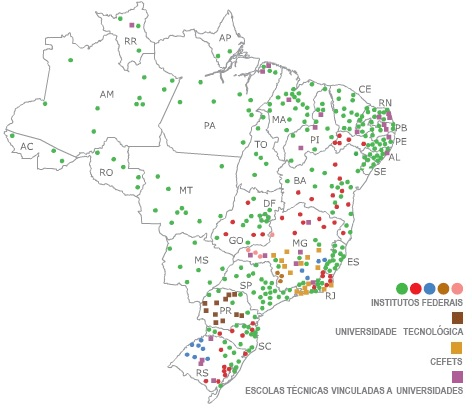
\includegraphics[width=0.8\textwidth, keepaspectratio]{rede.png}
	\legend{Adaptado de \citeonline{ifinstituicoes} pelo autor}
	\label{fig:rede}
\end{figure}

Seguindo as determinações da Lei nº 12.711 \cite{Lei12711}, as instituições da Rede Federal tem em sua política de seleção a reserva de 50\% das vagas a alunos oriundos integralmente do ensino médio público, sejam matriculados em cursos regulares ou da educação de jovens e adultos. Dessa reserva, metade delas estão destinadas para estudantes de escolas públicas com renda familiar bruta igual ou inferior a um salário mínimo e meio \textit{per capita}.

\subsection{Consulte o manual da classe \textsf{abntex2}}

Para exemplos adicionais de \abnTeX\ e \LaTeX, como inclusão de figuras,
fórmulas matemáticas, citações, e outros, consulte o documento
\citeonline{abntex2modelo}.

Consulte o manual da classe \textsf{abntex2} \cite{abntex2classe} para uma
referência completa das macros e ambientes disponíveis.

%\section{RESULTADOS}

%\section{Trabalhos relacionados}

% ---
% Finaliza a parte no bookmark do PDF, para que se inicie o bookmark na raiz
% ---
\bookmarksetup{startatroot}% 
% ---

% ---
% Conclusão
% ---
\section*{Considerações finais}
\addcontentsline{toc}{section}{Considerações finais}

\lipsum[2-4]

% ----------------------------------------------------------
% ELEMENTOS PÓS-TEXTUAIS
% ----------------------------------------------------------
\postextual

%\input{input/ingles.tex}

% ]  				% FIM DE ARTIGO EM DUAS COLUNAS
% ---

% ----------------------------------------------------------
% Referências bibliográficas
% ----------------------------------------------------------
\bibliography{references}

% ----------------------------------------------------------
% Glossário
% ----------------------------------------------------------
%
% Há diversas soluções prontas para glossário em LaTeX. 
% Consulte o manual do abnTeX2 para obter sugestões.
%
%\glossary

\end{document}
